\newpage
\section*{Figure e diagrammi}
%%%%%%%%%%%%%%%%%%%%%%%%%%%%%%%%%%%%%%%%%%%%%%%%%%%%%%%%%%%%
%%%%%%%%%%%%%%%%%%% Add here all figures %%%%%%%%%%%%%%%%%%%
\begin{figure}[h]
\centering
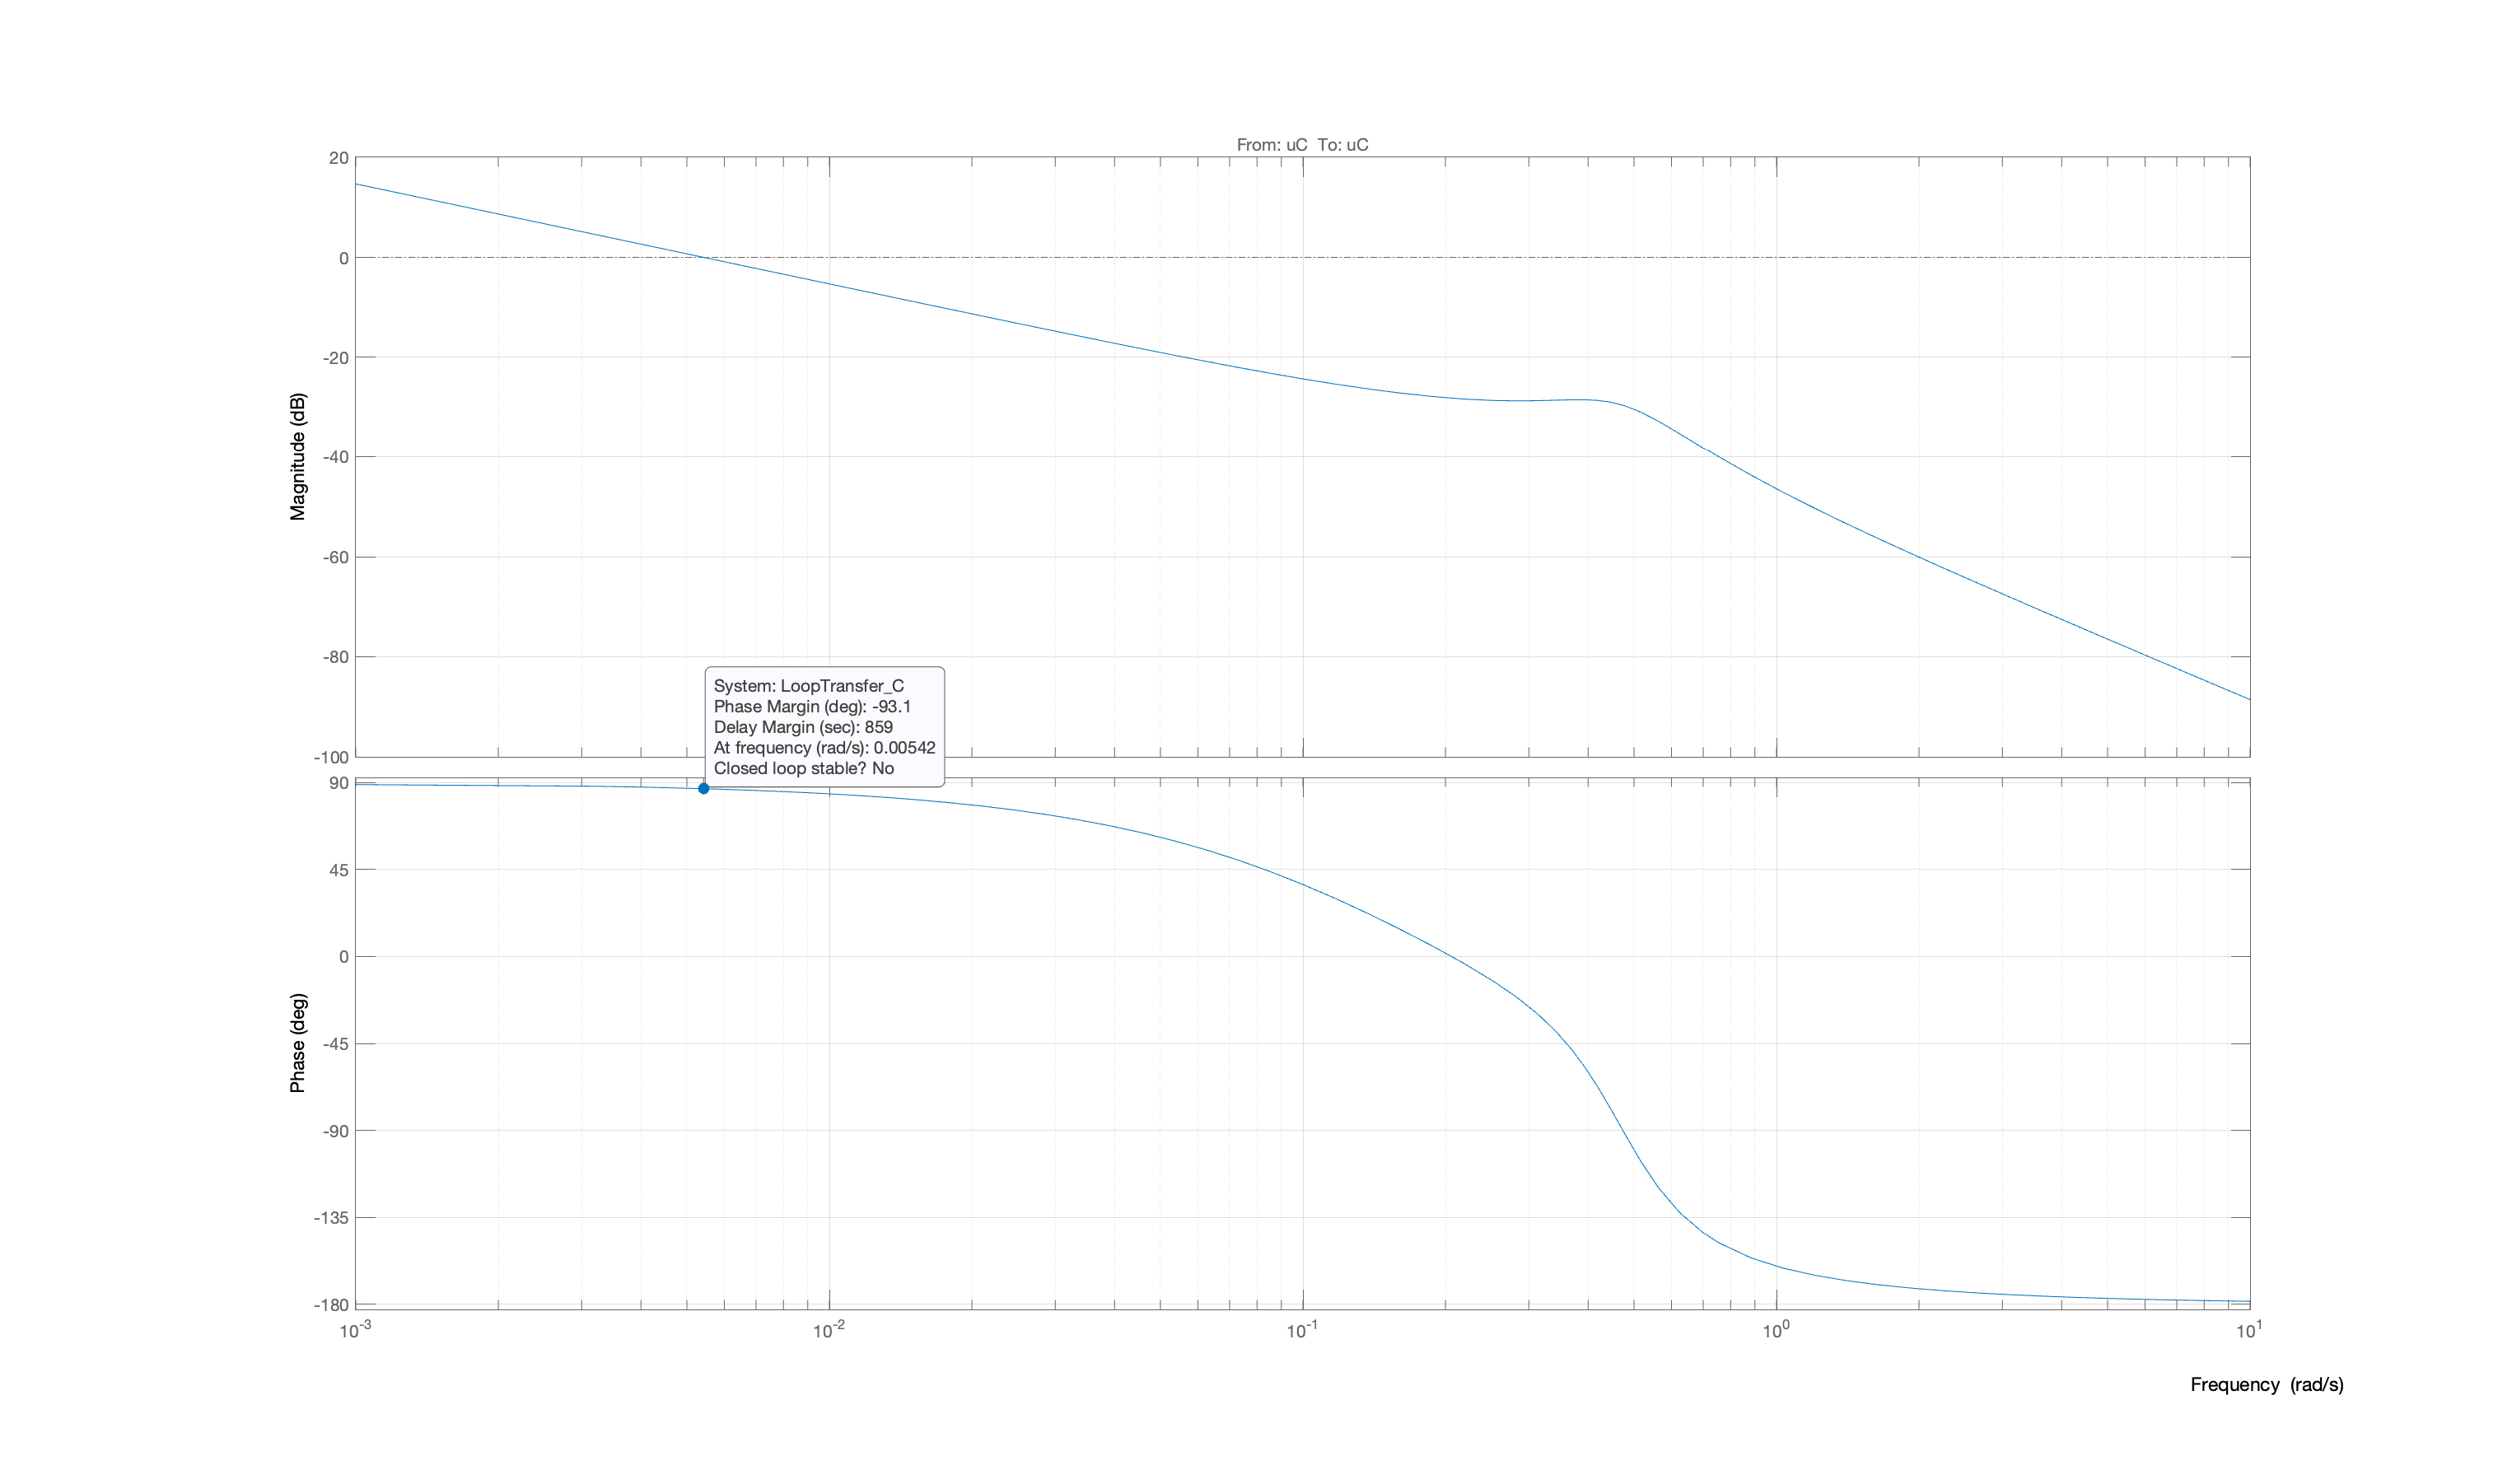
\includegraphics[width=0.85\columnwidth]{img/fig1.eps}
\caption{Diagrammi di Bode di $C(s) \, G(s)$ con $C(s)=1$.}
\label{fig:fig1}
\end{figure}

\begin{figure}[h]
\centering
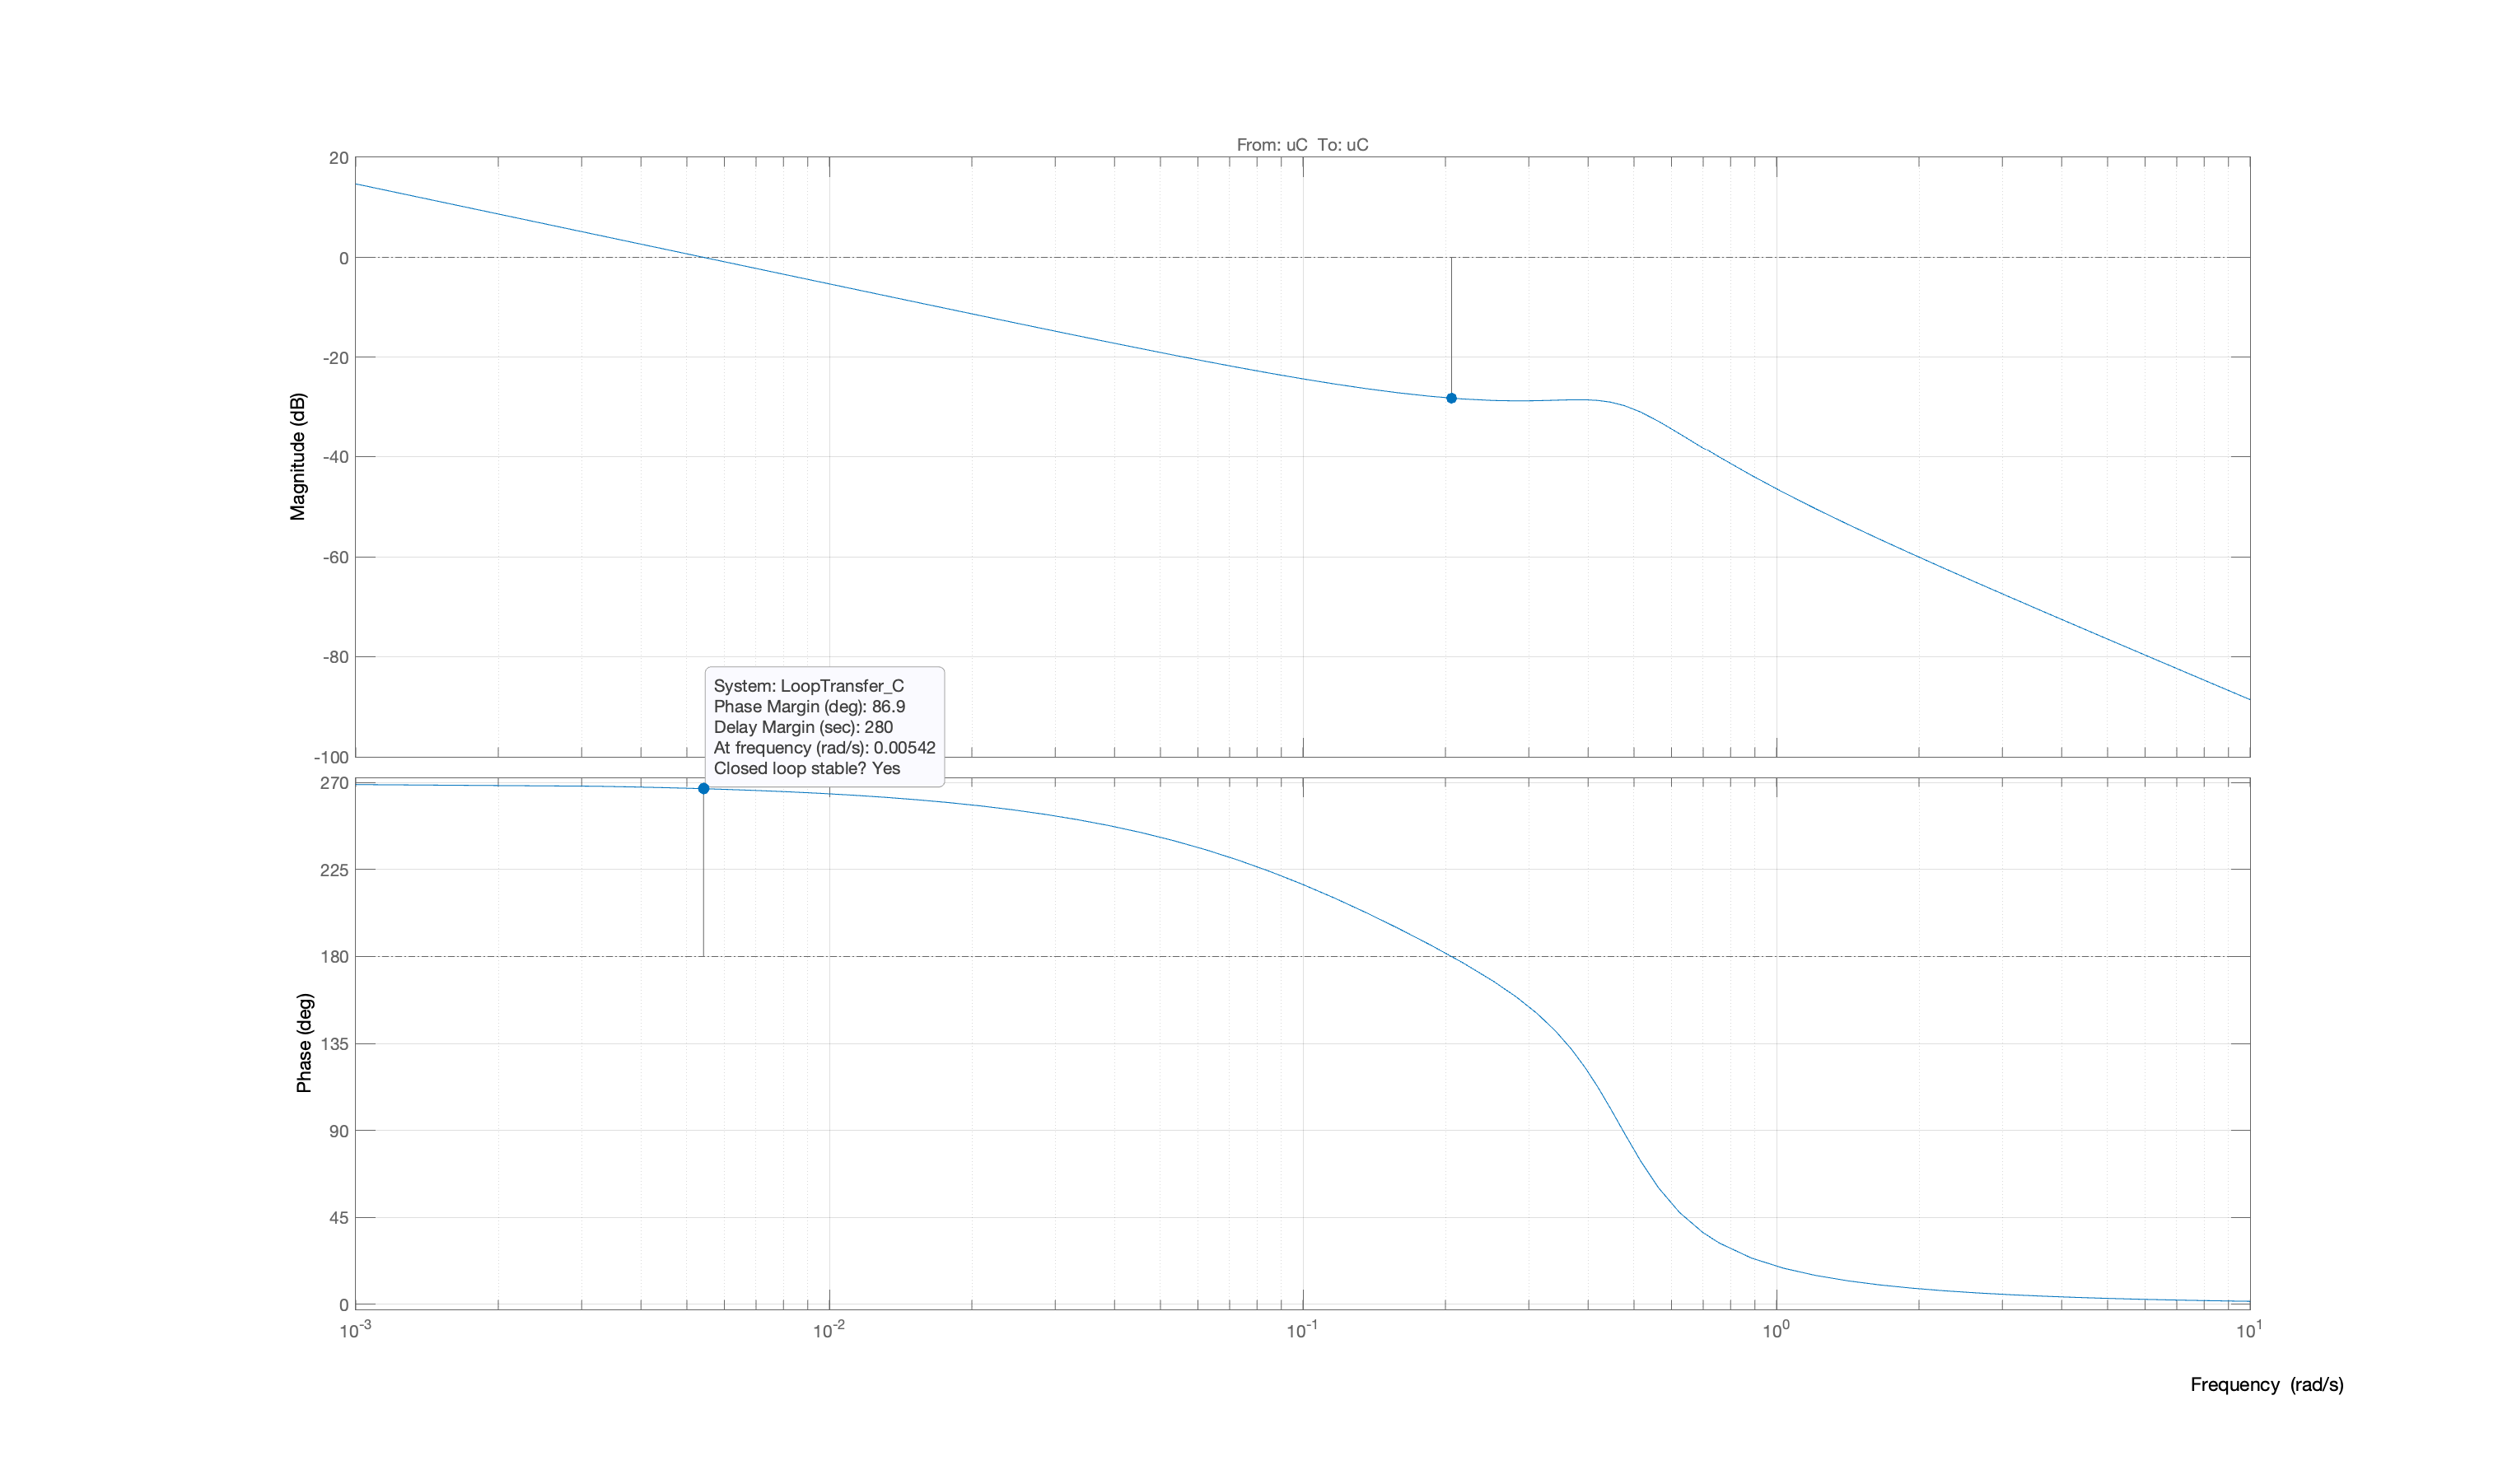
\includegraphics[width=0.85\columnwidth]{img/fig2.eps}
\caption{Diagrammi di Bode di $C(s) \, G(s)$ con $C(s)=-1$.}
\label{fig:fig2}
\end{figure}

\newpage

\begin{figure}[h]
\centering
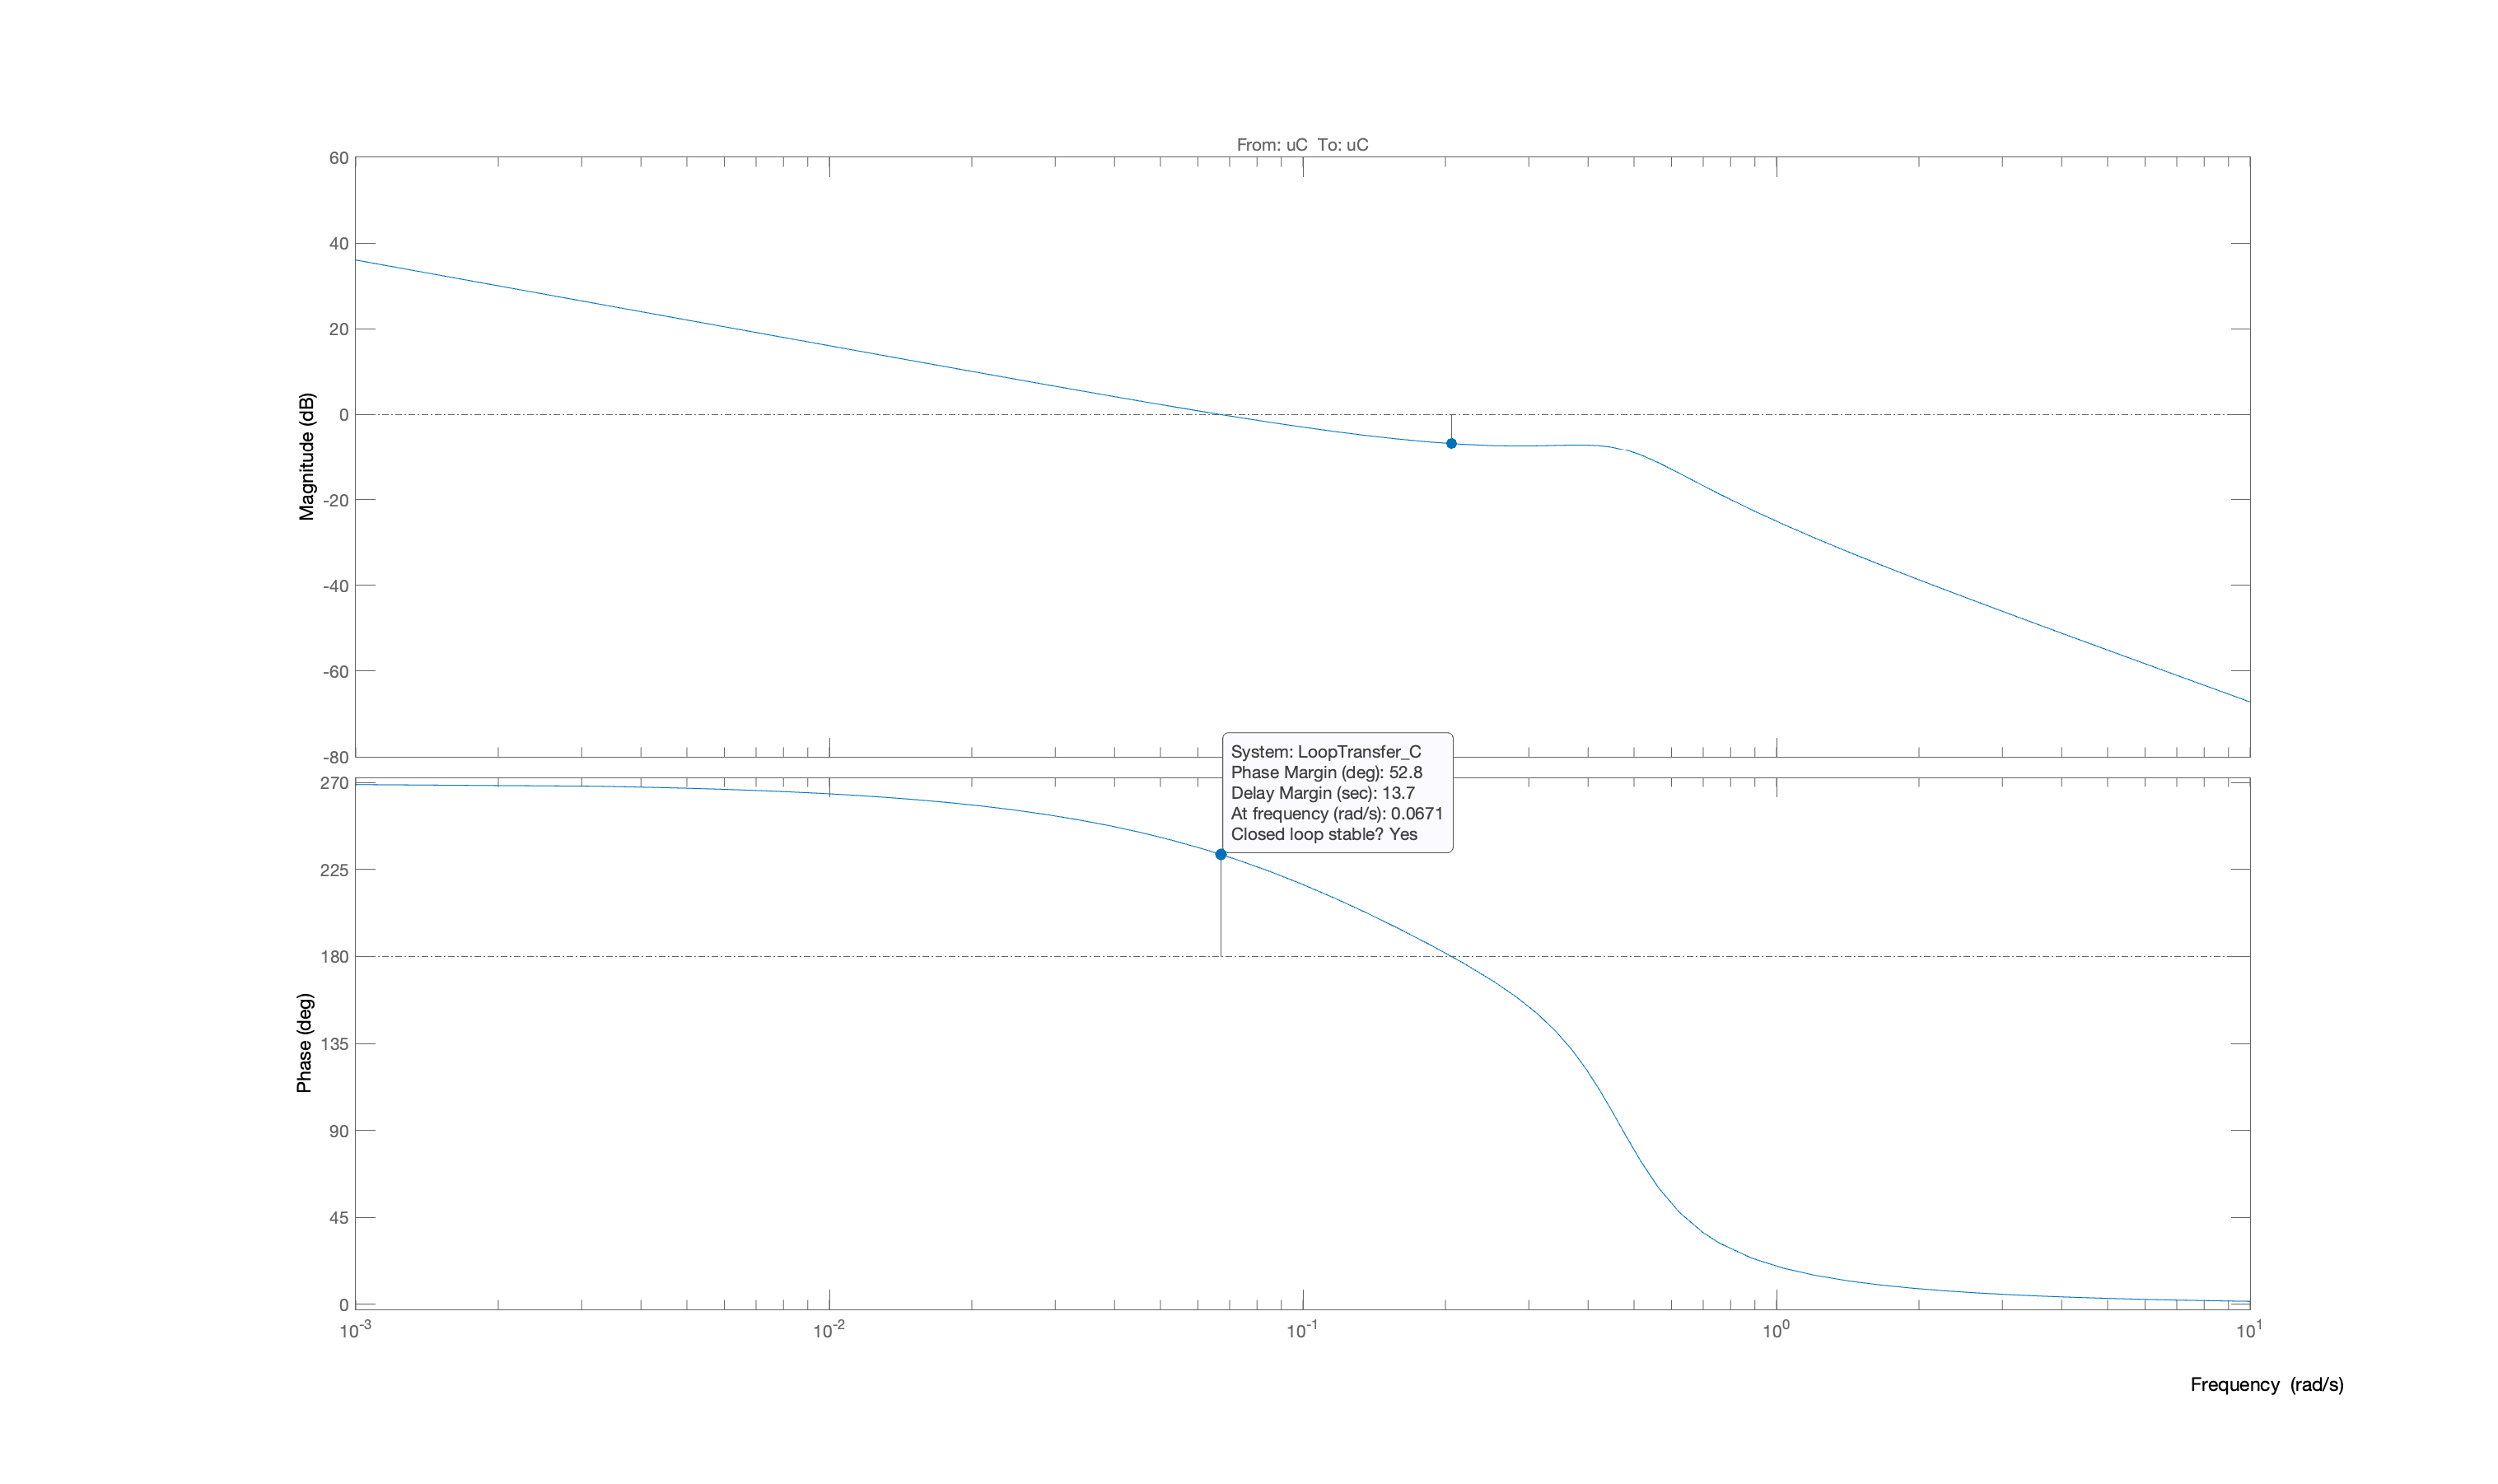
\includegraphics[width=0.85\columnwidth]{img/fig3.eps}
\caption{Diagrammi di Bode di $C(s) \, G(s)$ con $C(s)=-11.7$.}
\label{fig:fig3}
\end{figure}

\begin{figure}[h]
\centering
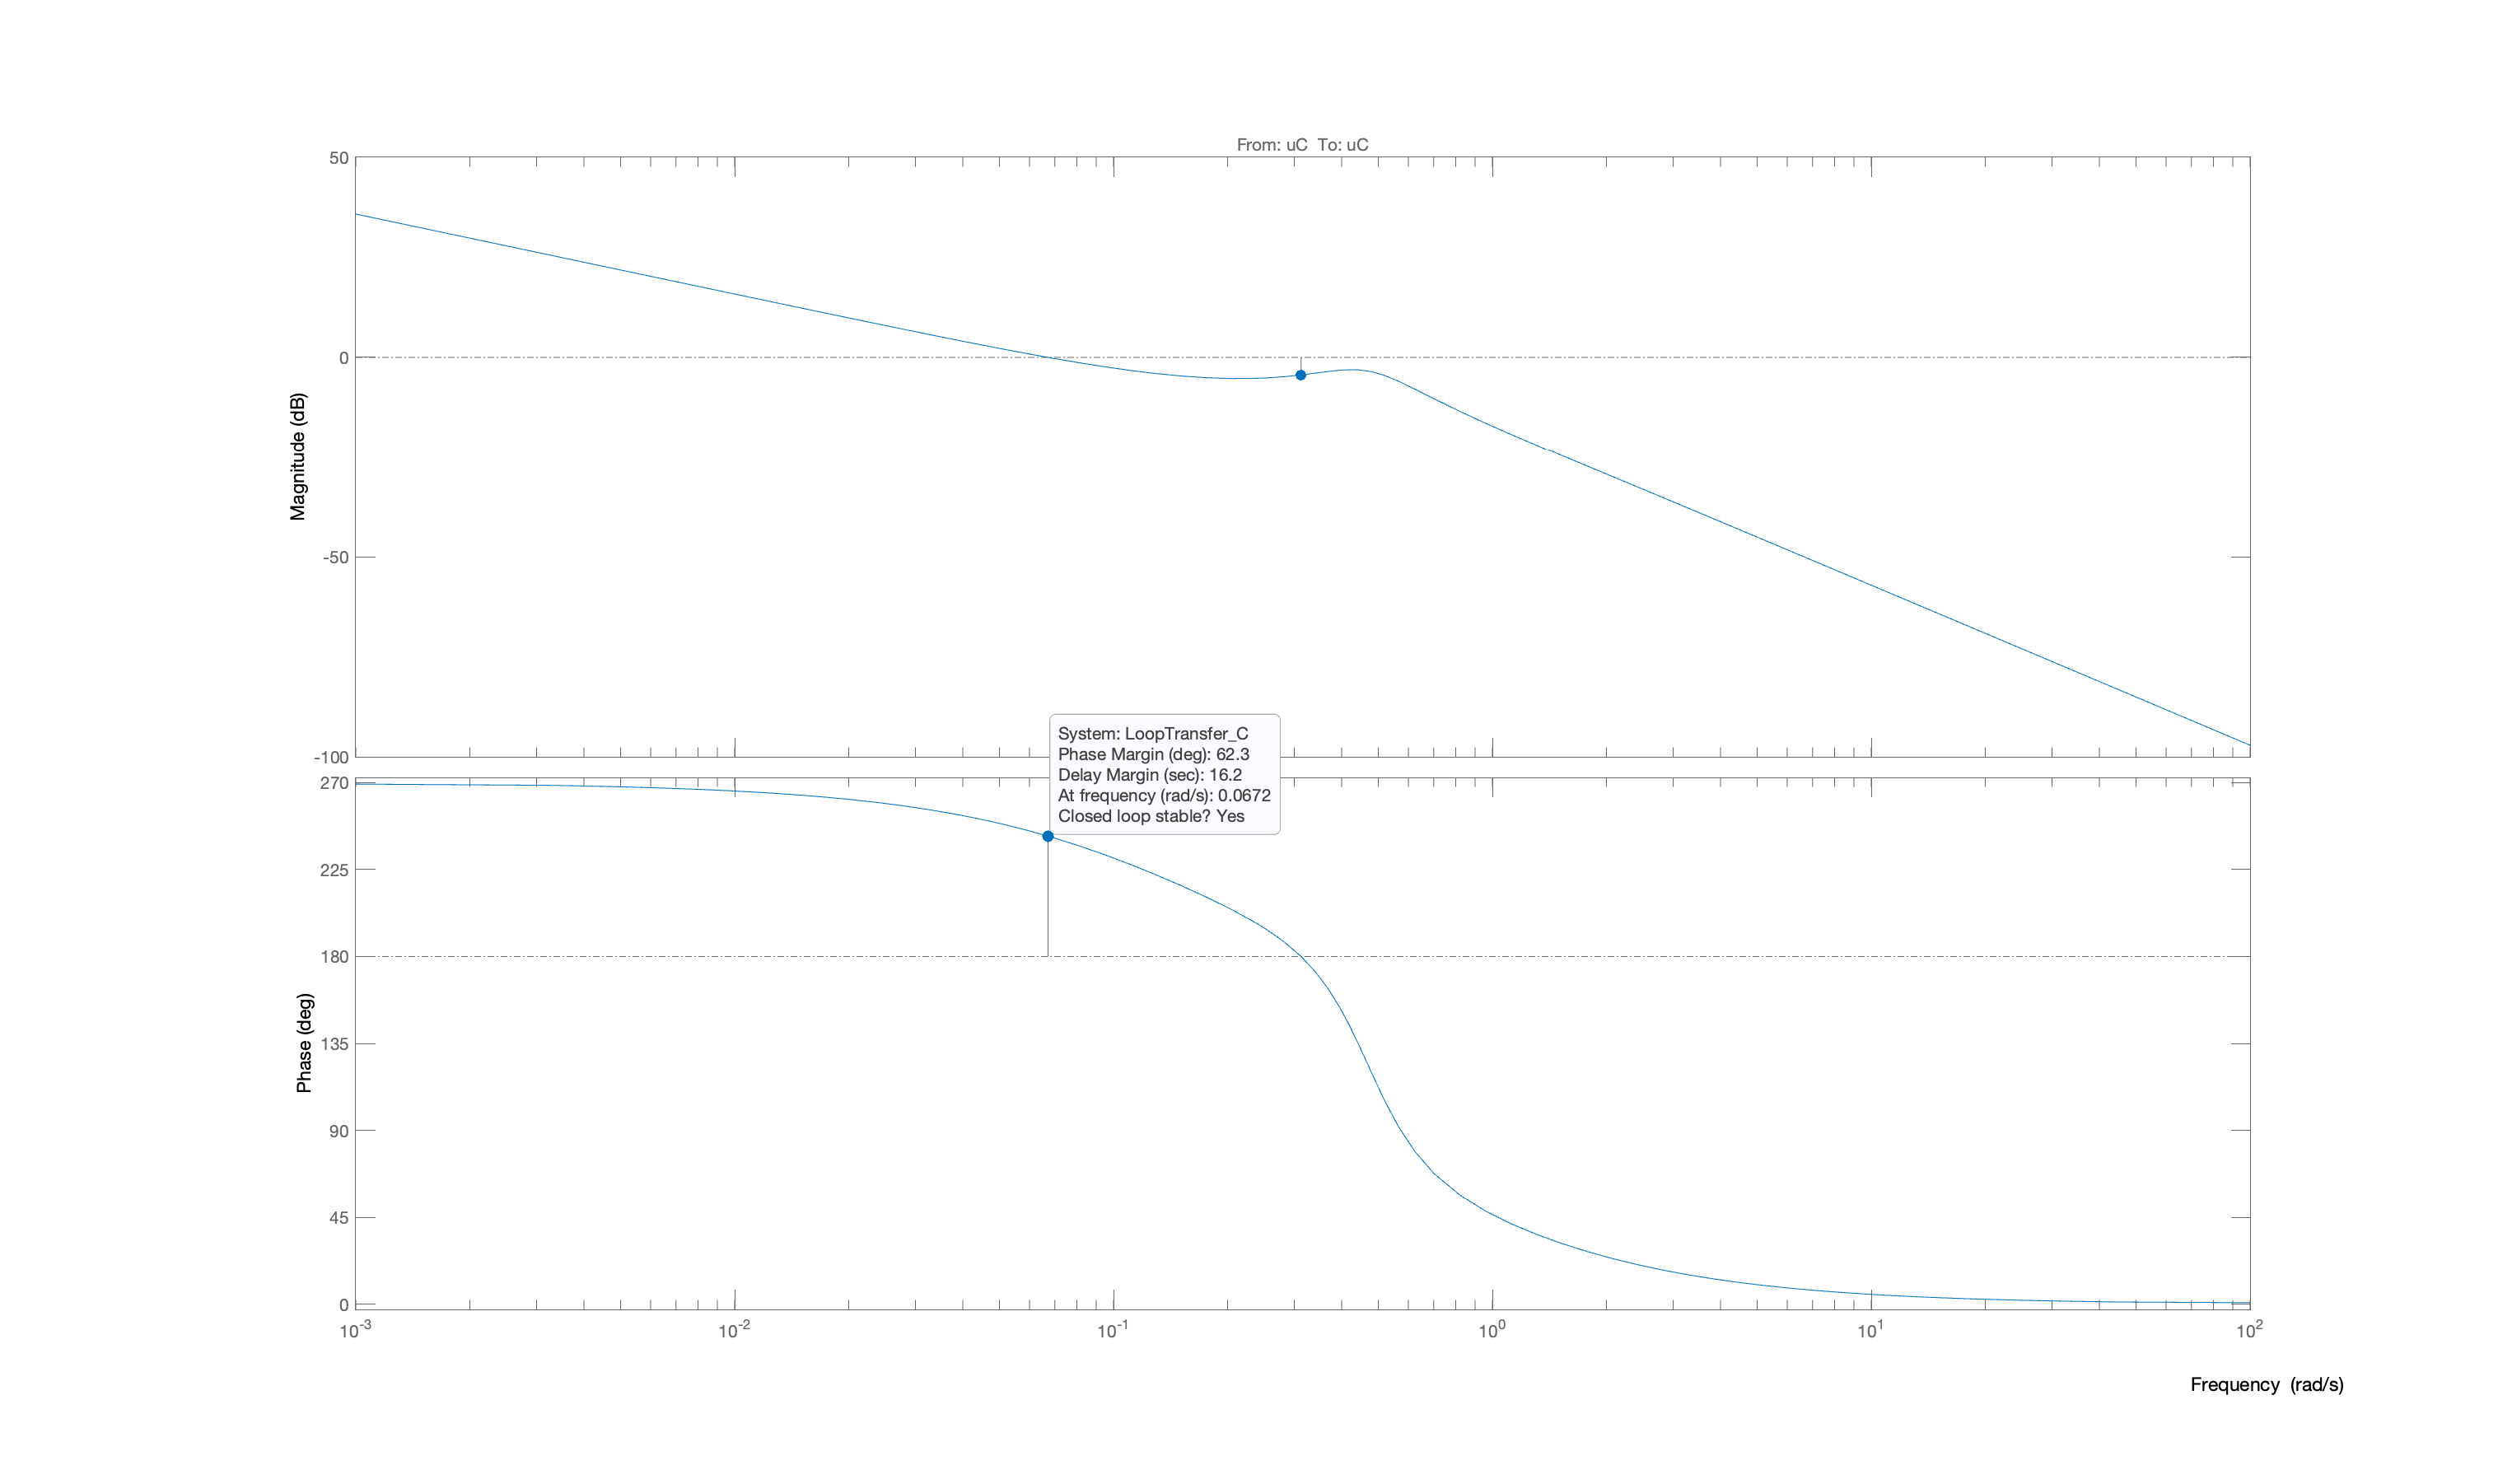
\includegraphics[width=0.85\columnwidth]{img/fig4.eps}
\caption{Diagrammi di Bode di $C(s) \, G(s)$ con $C(s)=-11.4 \, \frac{1+3.6s}{1+1.1s}$.}
\label{fig:fig4}
\end{figure}

\newpage

\begin{figure}[h]
\centering
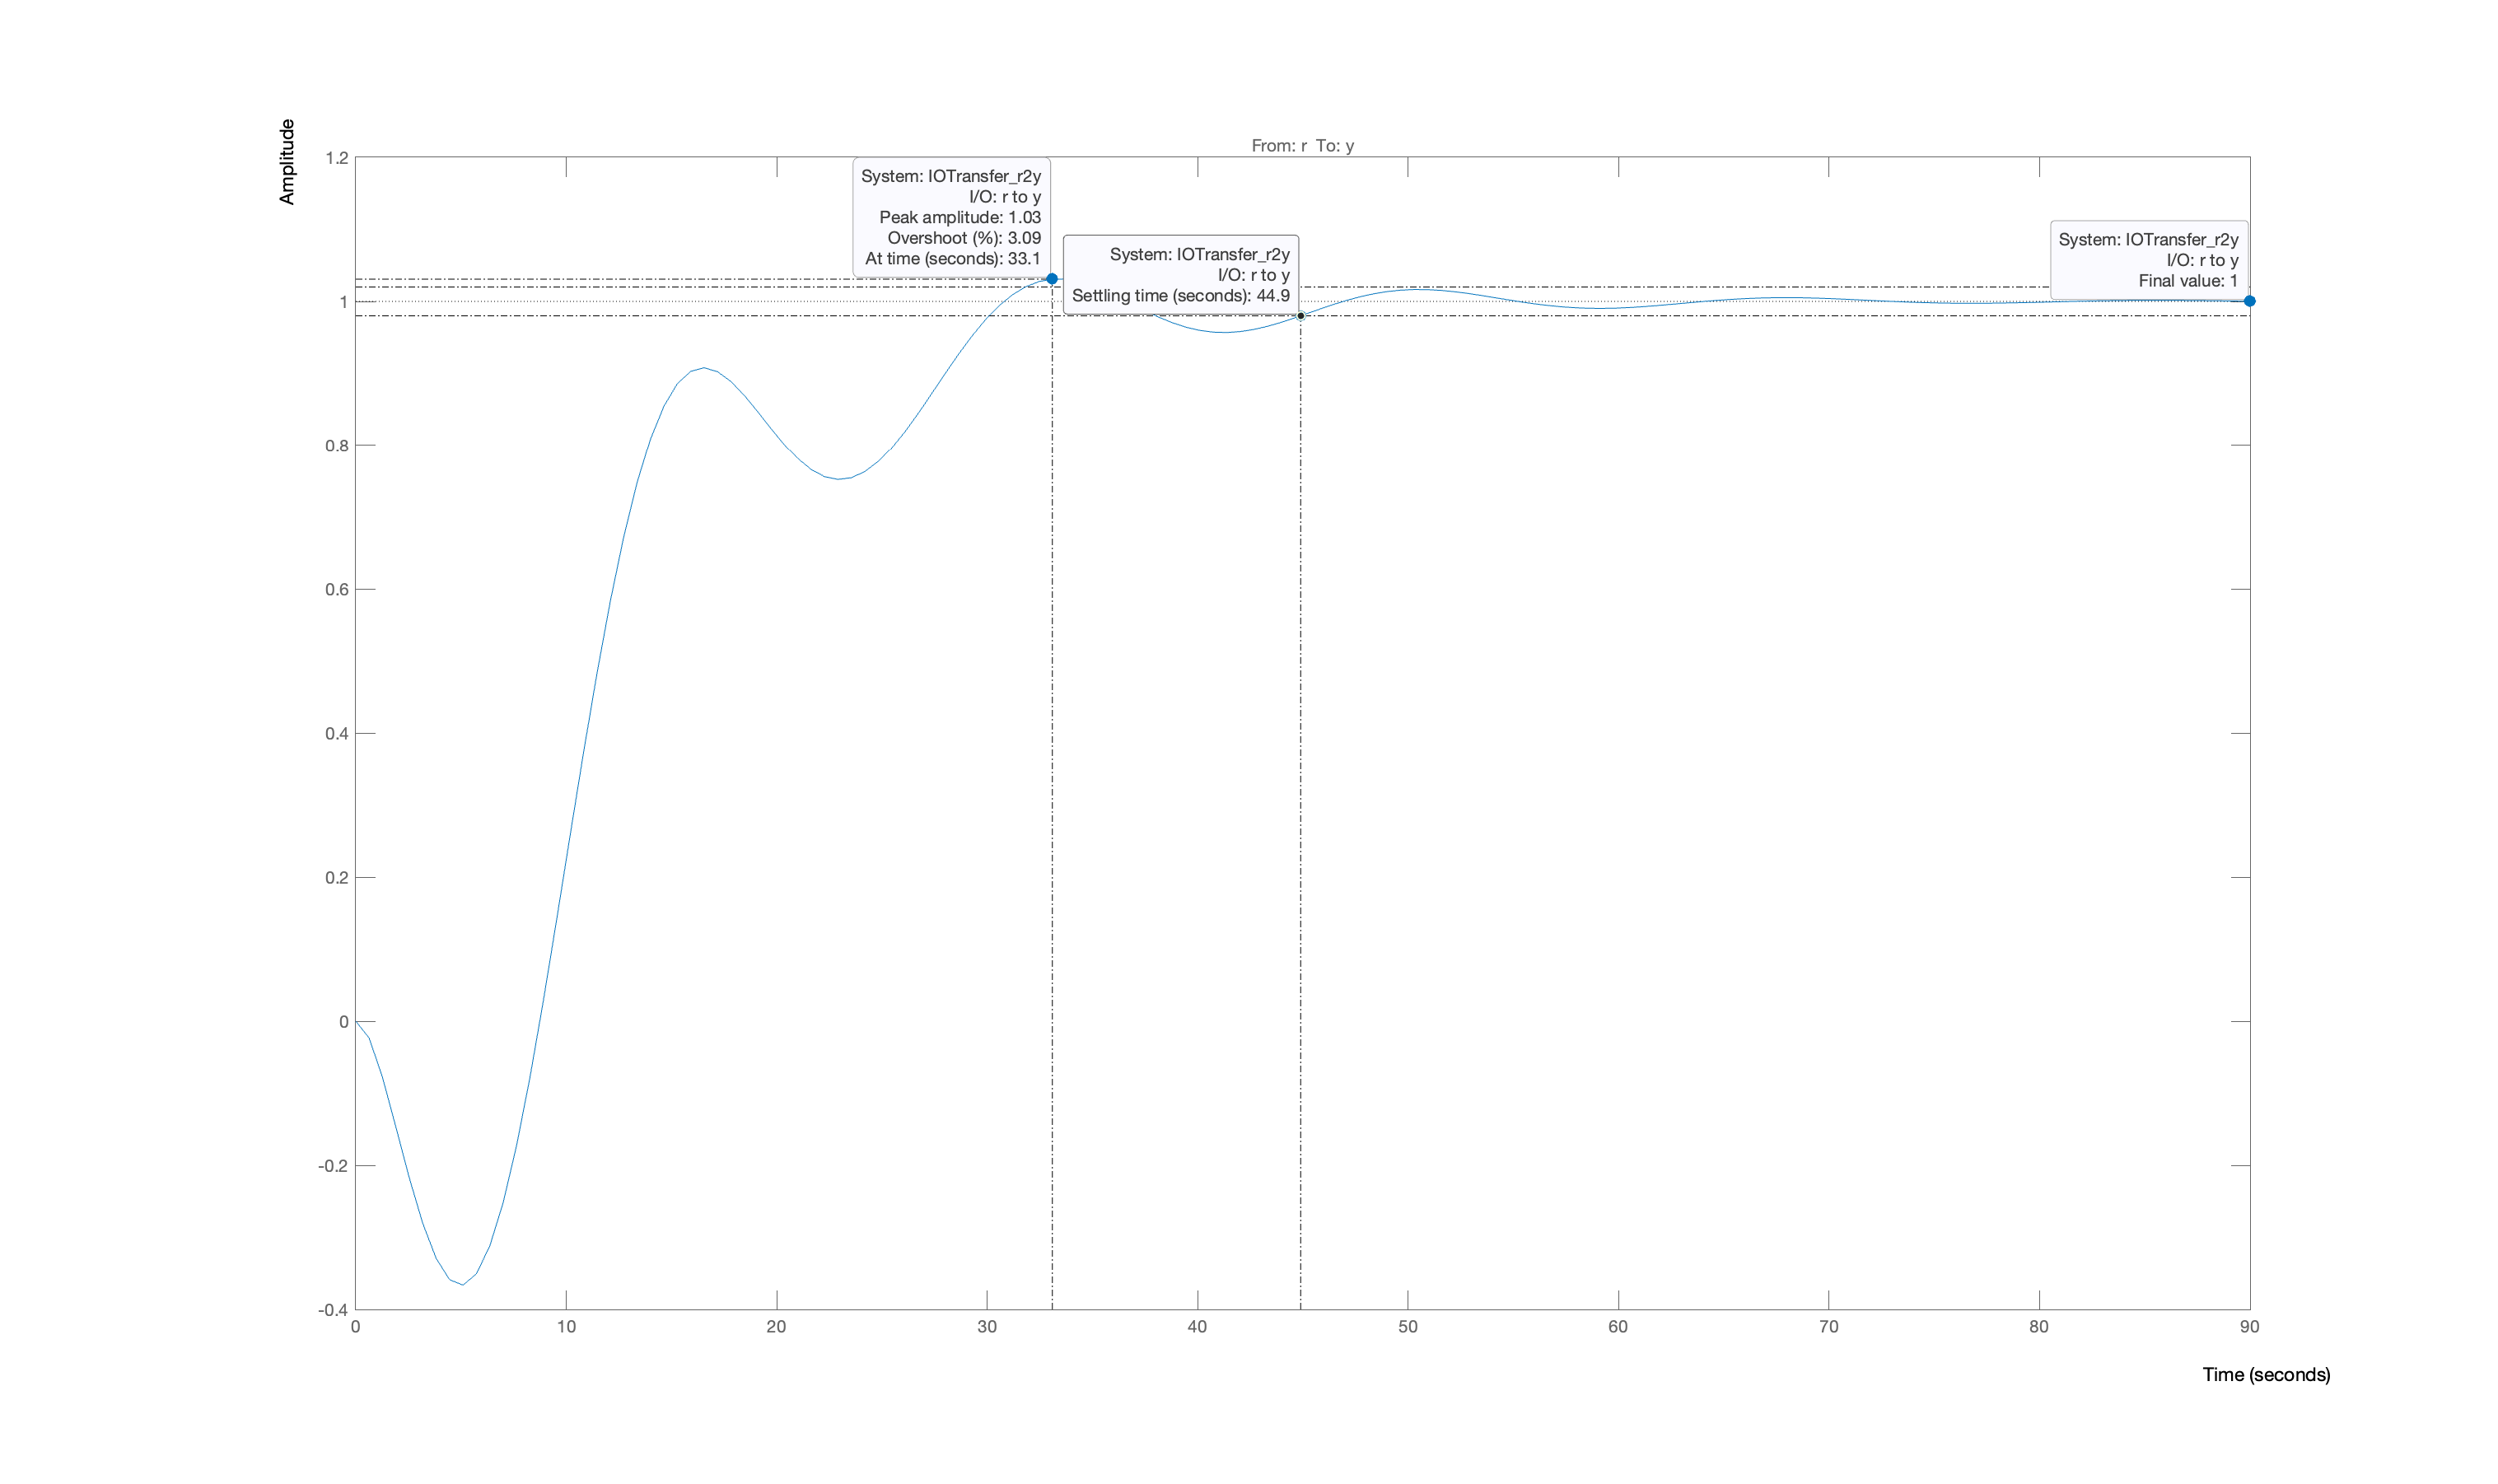
\includegraphics[width=0.85\columnwidth]{img/fig5.eps}
\caption{Risposta al gradino con caratteristiche indicate}
\label{fig:fig5}
\end{figure}

\begin{figure}[h]
\centering
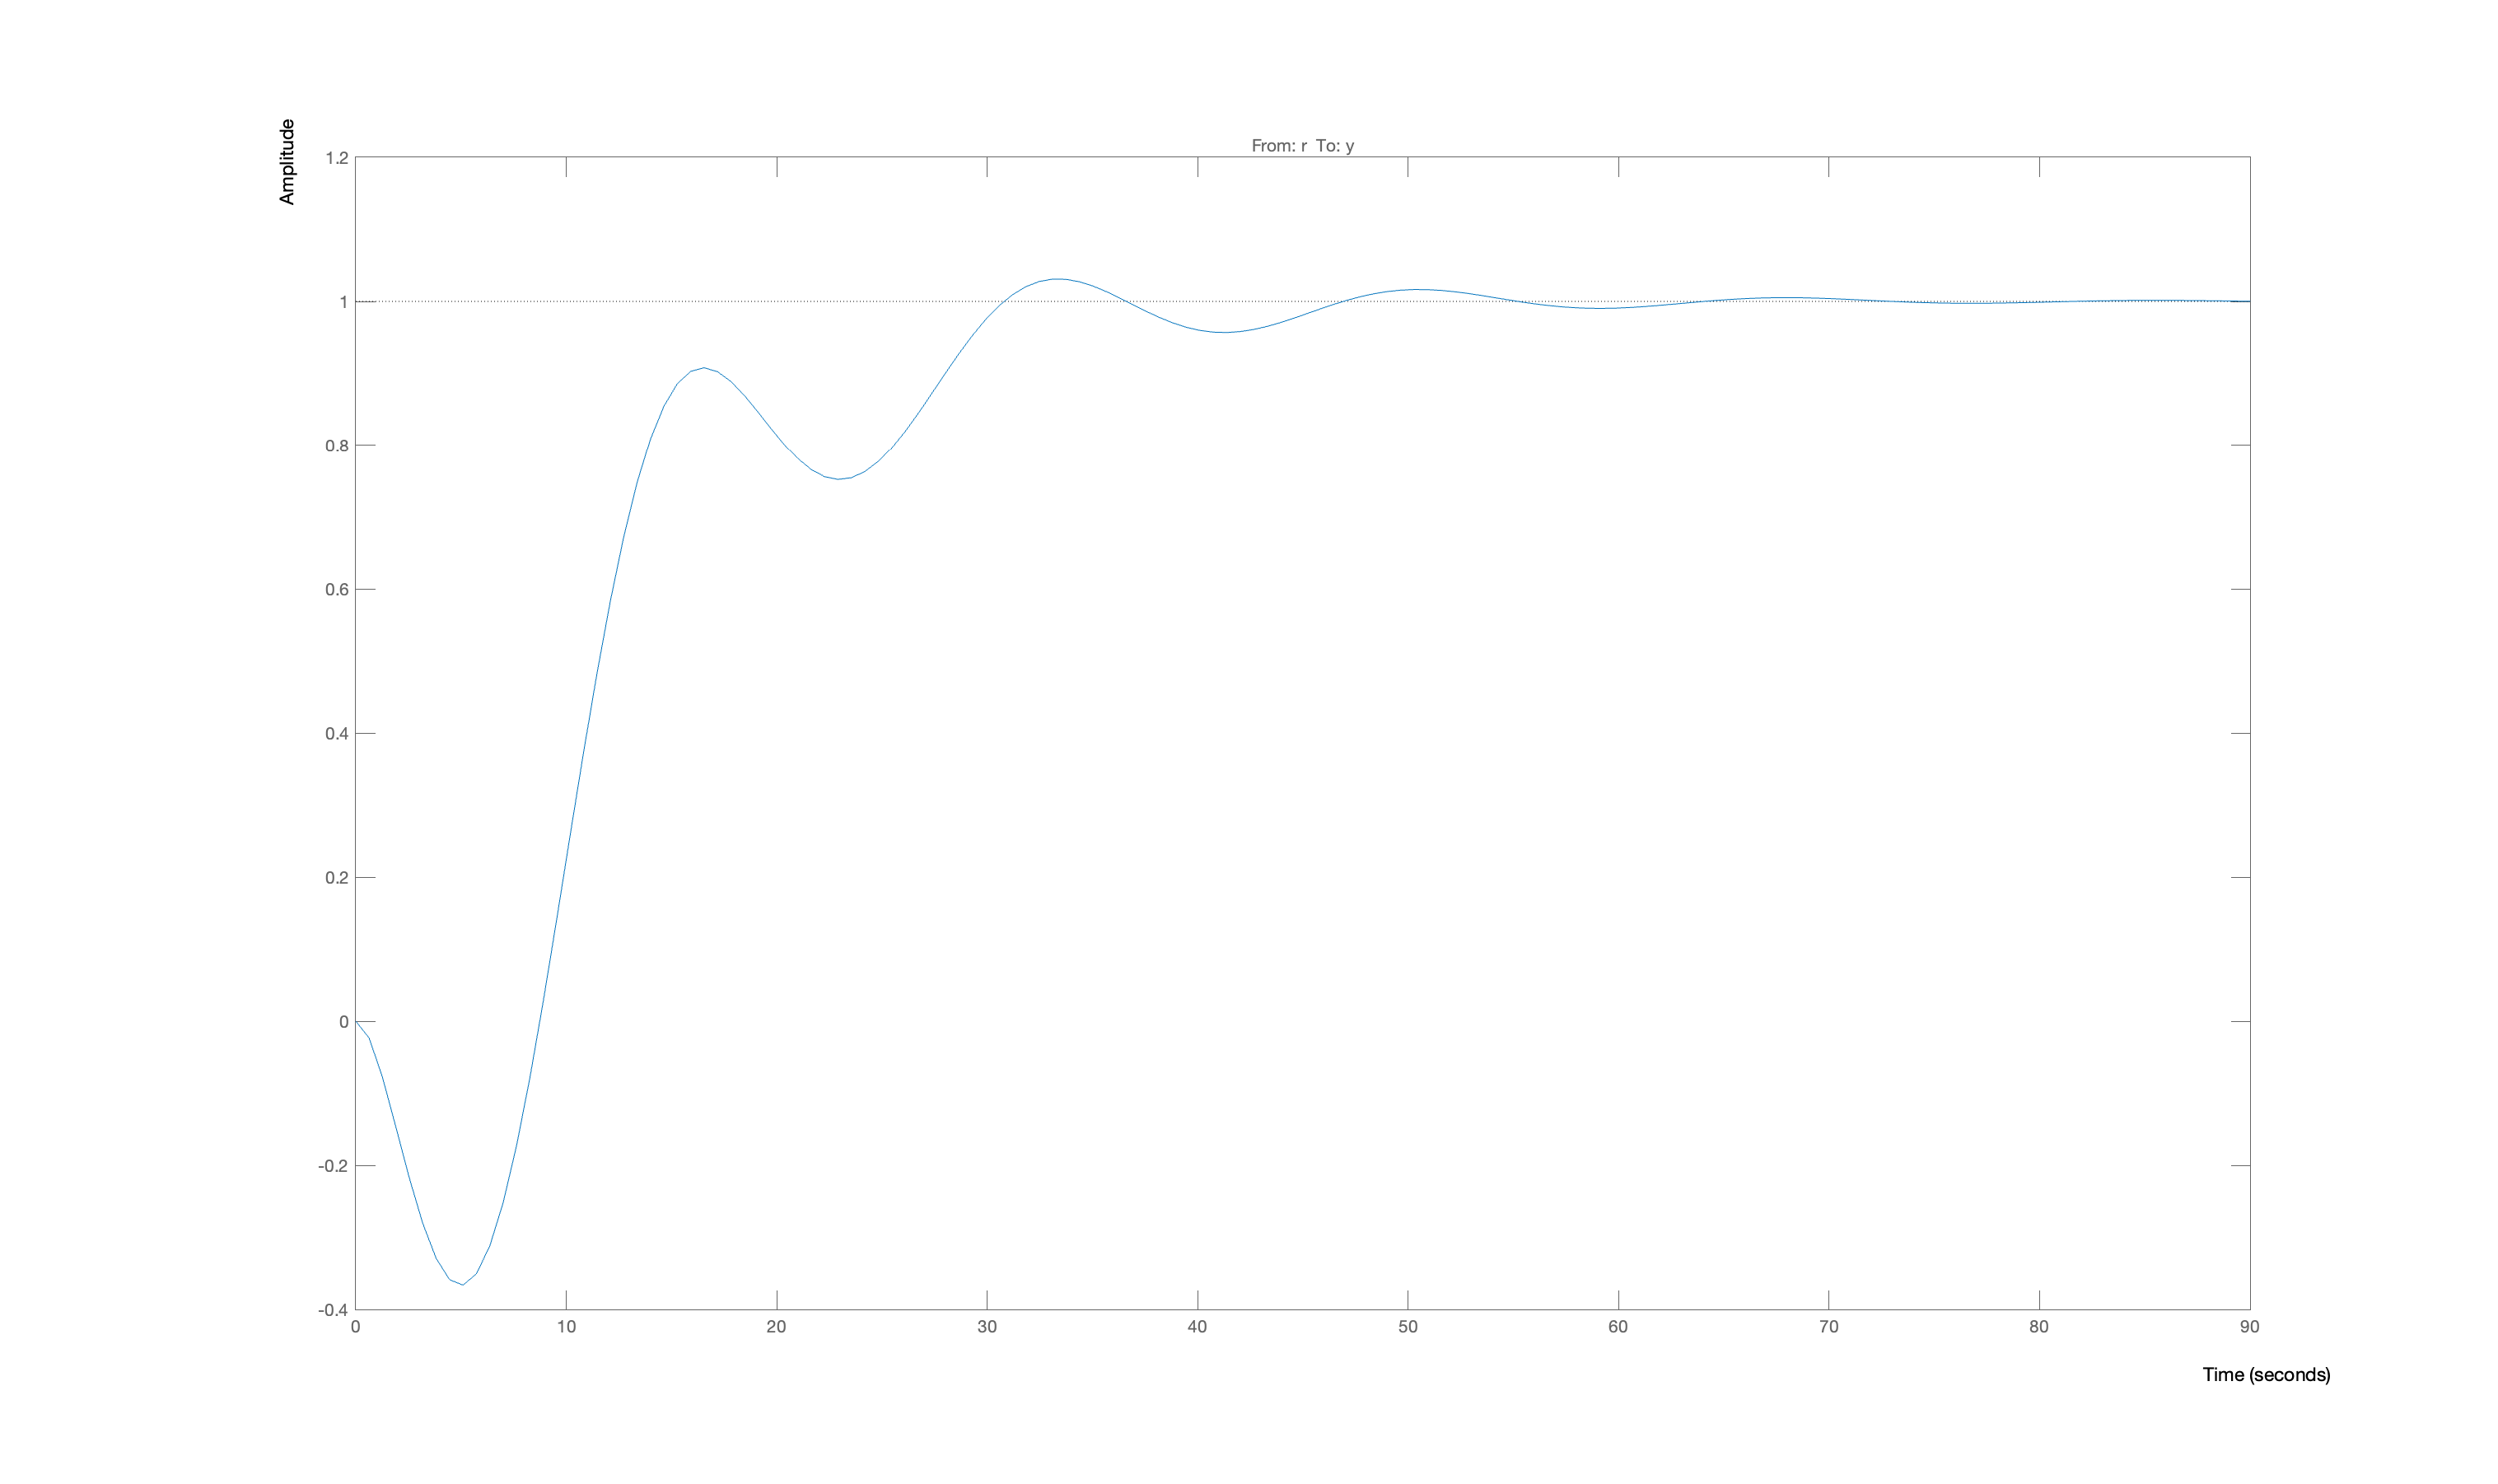
\includegraphics[width=0.85\columnwidth]{img/fig6.eps}
\caption{Risposta al gradino}
\label{fig:fig6}
\end{figure}

\newpage

\begin{figure}[h]
\centering
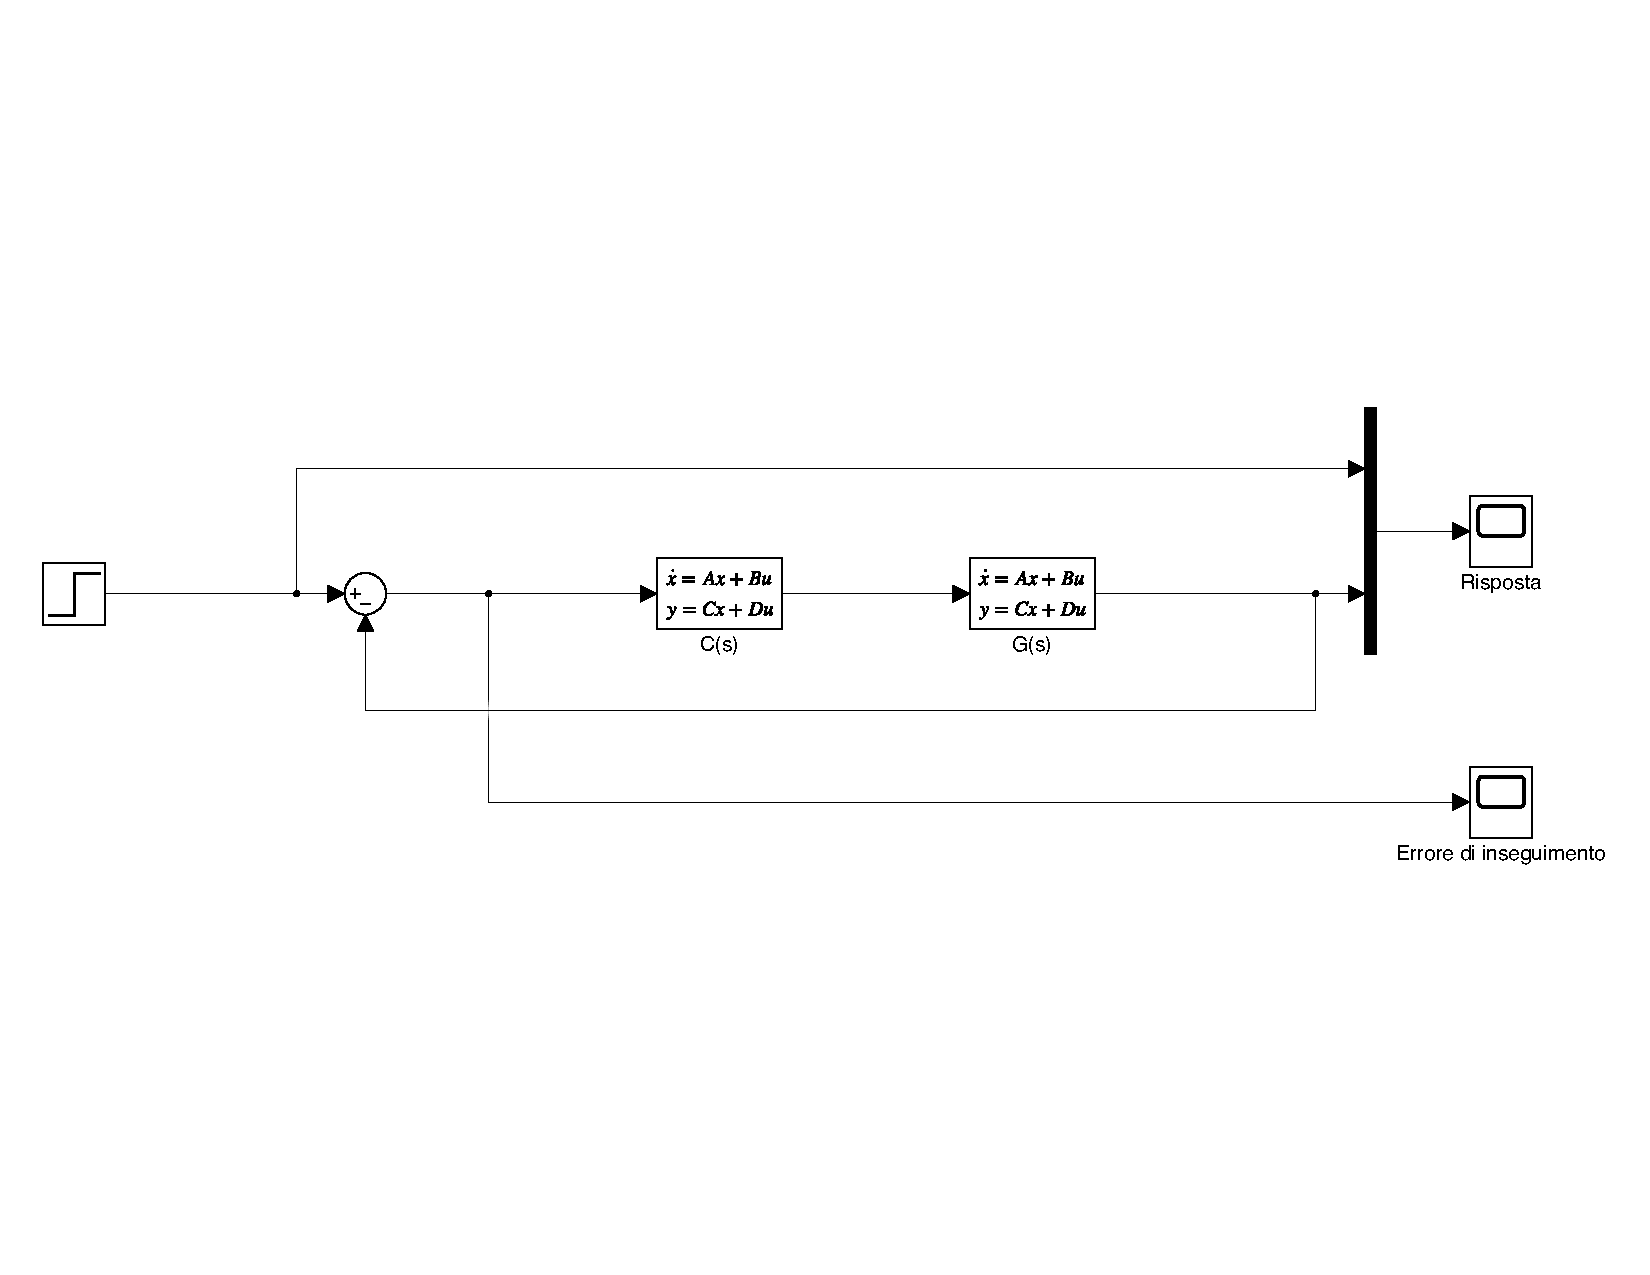
\includegraphics[width=1\columnwidth]{img/simulazione.pdf}
\caption{Schema Simulink che consente la simulazione e la verifica del soddisfacimento delle specifiche.}
\label{fig:simulink}
\end{figure}

\newpage

\begin{figure}[h]
\centering
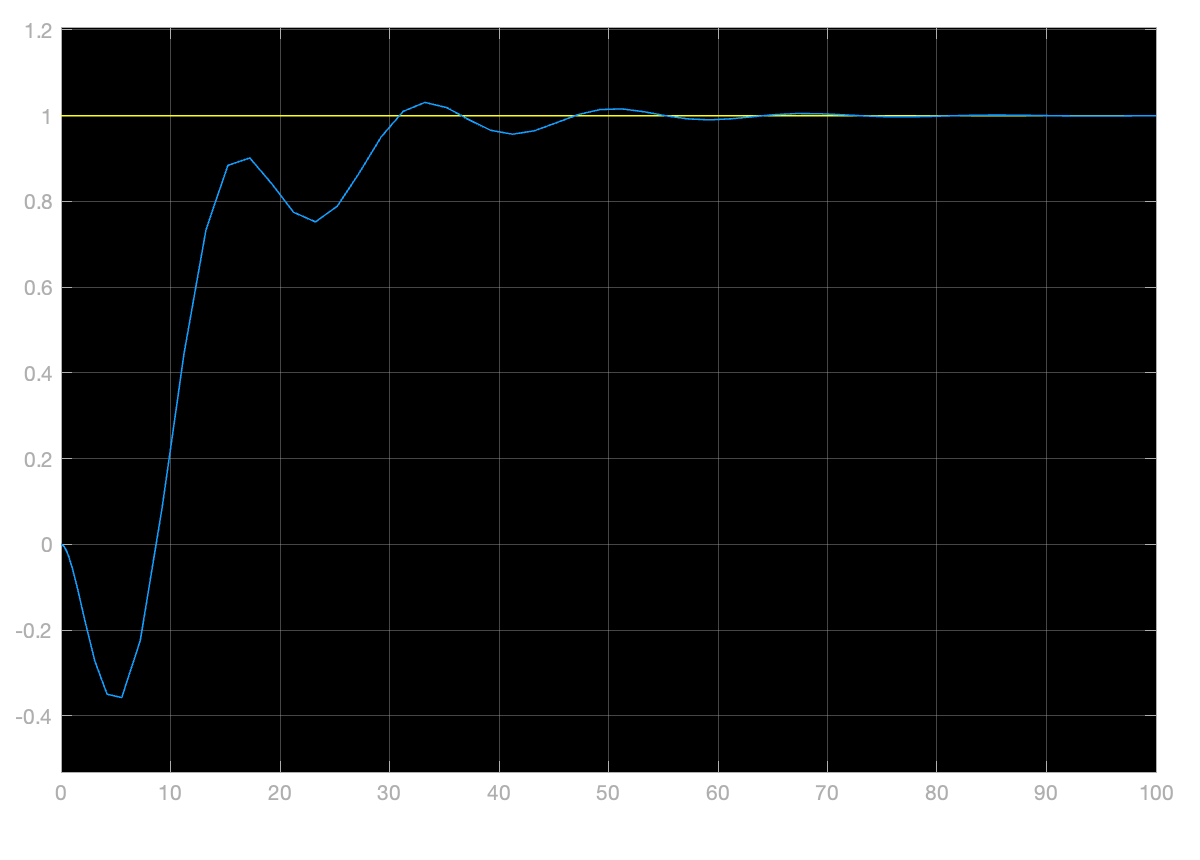
\includegraphics[width=1\columnwidth]{img/fig8.eps}
\caption{Risposta al gradino con Stop Time = 100s.}
\label{fig:fig8}
\end{figure}
%%%%%%%%%%%%%%%%%%%%%%%%%%%%%%%%%%%%%%%%%%%%%%%%%%%%%%%%%%%%
%%%%%%%%%%%%%%%%%%%%%%%%%%%%%%%%%%%%%%%%%%%%%%%%%%%%%%%%%%%%
